\section{Implementation}

\subsection{Code Style Configuration}
\begin{frame}[allowframebreaks]
\frametitle{Code Style Configuration}

The measurement component enforces some code styles:

\begin{itemize}
  \item Indentation levels
  \item Import statement styles
  \item Method name format
\end{itemize}

The code style is configurable using a JSON file:

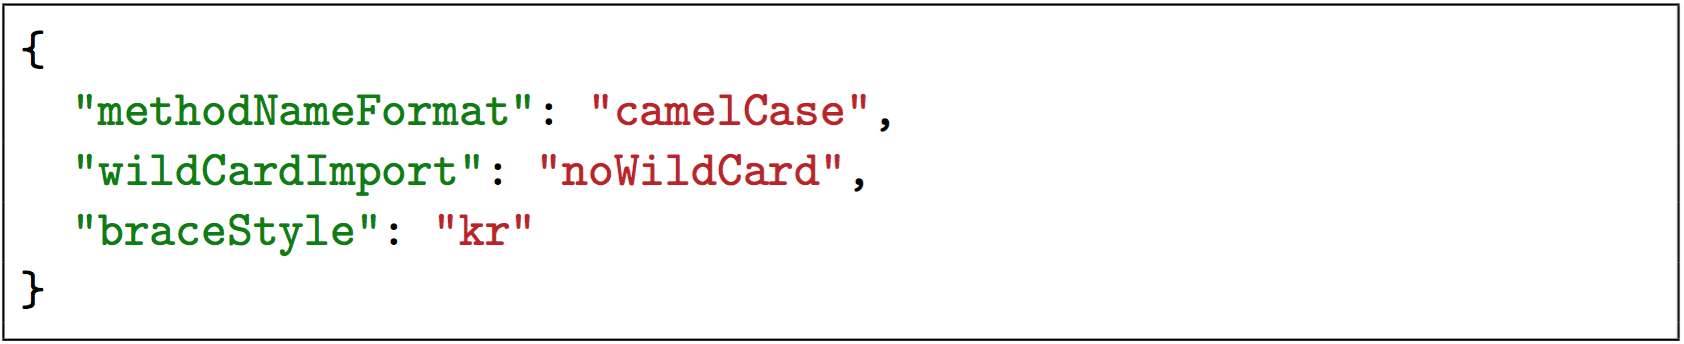
\includegraphics[scale=0.37]{json_config}

\framebreak

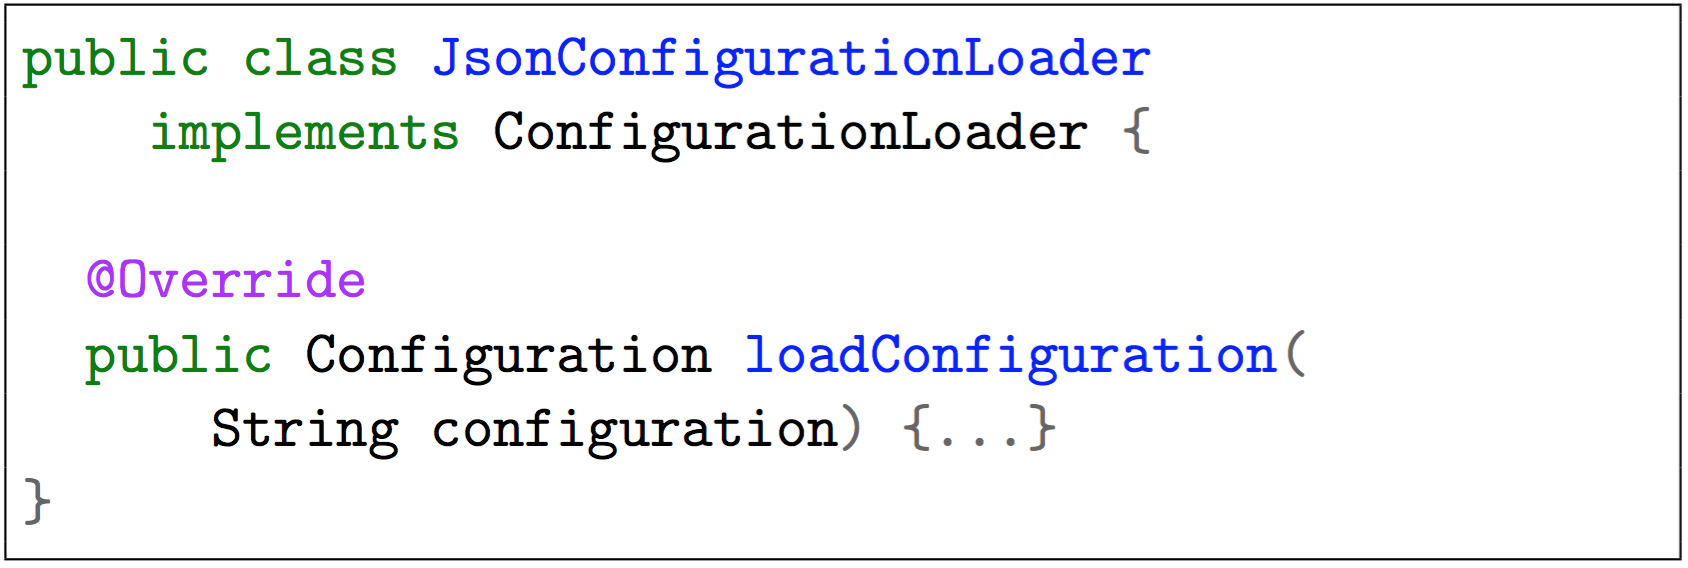
\includegraphics[scale=0.37]{json_configuration_loader}

Measurement component uses \textit{JsonConfigurationLoader} to convert the configuration in \textit{String} to \textit{Configuration} object.

We can implement the \textit{ConfigurationLoader} to support configuration XML and CSV formats.
\end{frame}

\subsection{Score Calculator}
\begin{frame}
\frametitle{Score Calculator}
\setbeamercovered{transparent}

\begin{columns}
\column{0.5\textwidth}
Washizaki et al. (2007) calculate scores based on \emph{benchmark} values and \emph{collected} values by using a linear piecewise function:
\begin{itemize}
  \item<1,4> If the collected value is less than benchmark value, the score is 100\%
  \item<2,4> If the collected value is more than benchmark value and less than 3 times of benchmark, the score is: $$score=\bigg(-\frac{1}{3 \times benchmark} \times value + \frac{4}{3}\bigg) \times 100\%$$
  \item<3,4> Else, the score is zero
\end{itemize}

\column{0.5\textwidth}
\begin{tikzpicture}
\begin{axis}[
    axis lines = left,
    xlabel = value,
    ylabel = score,
]
\addplot [
    domain=1:4, 
    samples=2,
    color=red,
]
{- x/3 + 4/3 };
\addplot [
    domain=0:1, 
    samples=2,
    color=red,
]
{1};
\addplot [
    domain=4:5, 
    samples=2,
    color=red,
]
{0};
\addplot [
    domain=0:1, 
    samples=2, 
    color=white,
]
{1.1};
\end{axis}
\end{tikzpicture}

\end{columns}

\end{frame}

\subsection{Front-end Development}
\begin{frame}
\frametitle{Front-end Development}
To enhance user experience, we built a single page application for front-end of SQAT:
\begin{itemize}
  \item Contents are loaded dynamically using Javascript
  \item URL is changed to emulate traditional navigation
\end{itemize}

We uses Flux Architecture for front-end application:

\begin{tikzpicture}[
squarednode/.style={rectangle, draw=black!60, very thick, minimum size=1cm},
]
%Nodes
\node[squarednode](action){Action};
\node[squarednode](dispatcher)[right=of action]{Dispatcher};
\node[squarednode](store)[right=of dispatcher]{Store};
\node[squarednode](view)[right=of store]{View};

\node[squarednode](action2)[above=of store]{Action};

%Lines
\draw[->] (action.east) -- (dispatcher.west);
\draw[->] (dispatcher.east) -- (store.west);
\draw[->] (store.east) -- (view.west);

\draw[->] (view.north) -- (action2.east);
\draw[->] (action2.west) -- (dispatcher.north);
\end{tikzpicture}

\end{frame}